\documentclass[12pt,a4paper]{report}
\usepackage[left=1.5in,right=1in,top=1in,bottom=1in]{geometry}
\usepackage[colorlinks=true,linkcolor=blue,urlcolor=blue,citecolor=blue]{hyperref}
\usepackage{natbib}
\usepackage{epsfig}
\usepackage{amsmath}
\usepackage{microtype}
\usepackage{booktabs}
\usepackage{tabularray}
\usepackage{placeins}
\usepackage{epstopdf}
\usepackage{pdflscape}
\usepackage{setspace}
\usepackage{enumerate}
\usepackage{rotating}
\usepackage{color}
\usepackage{caption}
\usepackage{float}
\usepackage{longtable}
\onehalfspacing
\usepackage{fancyhdr}
\setlength{\headheight}{28pt}
\usepackage[svgnames]{xcolor}
\usepackage[toc,page]{appendix}
\usepackage{rotating}
\usepackage{pdflscape}
\usepackage{tabulary}  
\usepackage{multirow} 
\usepackage{csquotes}
\usepackage{graphics}
\usepackage{booktabs, tabularx}
\usepackage{ragged2e}
\newcolumntype{L}{>{\RaggedRight}X}
\usepackage{enumitem}
\renewcommand{\arraystretch}{1}
\pagestyle{fancy}
\fancyhf{}
%\renewcommand{\headrulewidth}{1pt}
\fancyhead[L]{\textbf{\nouppercase{\leftmark}}}
\fancyhead[R]{\textbf{\thepage}}
\renewcommand\bibname{References}
\doublespacing
\urlstyle{same}
\newtheorem{remark}{Remark}
\newtheorem{lemma}{Lemma}
\makeatletter
\newenvironment{chapquote}[2][2em]
{\setlength{\@tempdima}{#1}%
\def\chapquote@author{#2}%
\parshape 1 \@tempdima \dimexpr\textwidth-2\@tempdima\relax%
\itshape}
{\par\normalfont\hfill--\ \chapquote@author\hspace*{\@tempdima}\par\bigskip}
\makeatother
\usepackage{listings}
\usepackage{xcolor}
\lstset{language=R,
	basicstyle=\small\ttfamily,
	stringstyle=\color{skyblue},
	otherkeywords={0,1,2,3,4,5,6,7,8,9},
	morekeywords={TRUE,FALSE},
	deletekeywords={data,frame,length,as,character},
	keywordstyle=\color{blue},
	commentstyle=\color{DarkGreen},
}

\definecolor{codegreen}{rgb}{0,0.6,0}
\definecolor{codegray}{rgb}{0.5,0.5,0.5}
\definecolor{codepurple}{rgb}{0.58,0,0.82}
\definecolor{backcolour}{rgb}{0.95,0.95,0.92}

\lstdefinestyle{mystyle}{
	backgroundcolor=\color{backcolour},   
	commentstyle=\color{DarkGreen},
	keywordstyle=\color{blue},
	numberstyle=\tiny\color{codegray},
	stringstyle=\color{purple},
	basicstyle=\small\ttfamily,
	breakatwhitespace=false,         
	breaklines=true, captionpos=b,                    
	keepspaces=true, numbers=left,                    
	numbersep=5pt, showspaces=false,                
	showstringspaces=false, showtabs=false, tabsize=2}
\lstset{style=mystyle}
\graphicspath{{./ThesisPlots/}}

\begin{document}
	
\begin{titlepage}
\vspace{10cm}
\begin{center}
\large
\begin{center}
\textbf{
YOUR THESIS TITLE IS WRITTEN HERE...
} \\
\end{center}
\vspace{0.3cm}
\begin{figure}[htbp]
\centering

\includegraphics[width=10cm]{Logo.jpg}
\label{fig:mono}
\end{figure}
\vspace{1cm}
\large
\textbf{%[0.8\baselineskip]
By\\%[0.2\baselineskip]
Author Name
}\\ %[0.8\baselineskip]\\
{\normalsize}  
\vspace{2.5cm}
\large
\textbf{
Department of Statistics\\
Faculty of Natural Sciences\\
Quaid-i-Azam University, Islamabad\\
2022
}
\end{center}
\end{titlepage}

\newpage
\pagenumbering{roman}
\setcounter{page}{1}
\vspace*{3.5cm}
\begin{figure}[htbp]
\centering

\includegraphics[scale=0.20]{Bismillah.png}
\label{fig:bism}
\end{figure}
\vspace{0.5cm}
\large
\begin{center}
\textit{In the Name of Allah
The Most Merciful and The Most Beneficent}\\
\end{center}
\vspace{0.3cm}
\begin{center}
\newpage
\vspace{10cm}
\begin{center}
\large
\begin{center}
\textbf{
YOUR THESIS TITLE IS WRITTEN HERE...
}
\end{center}
\vspace{0.3cm}
\begin{figure}[htbp]
\centering

\includegraphics[width=8cm]{Logo.jpg}
\label{fig:QAU-mono}
\end{figure}
\large
\textbf{%[0.8\baselineskip]
By\\%[0.2\baselineskip]
Author Name
}\\%[0.8\baselineskip]\\
{\normalsize}
\vspace{1cm}
\small
\textit{
A THESIS SUBMITTED IN THE PARTIAL FULFILLMENT OF THE REQUIREMENTS FOR THE DEGREE OF MASTER OF PHILOSOPHY IN STATISTICS
}\\
\vspace{0.5cm}
\large
\textbf{Supervised By\\
Name of supervisor}\\
\vspace{0.5cm}
\large

\textbf{Department of Statistics\\
Faculty of Natural Sciences\\
Quaid-i-Azam University, Islamabad\\
2022}
\end{center}
\end{center}
	
 \newpage
	
 \vspace*{2.2 cm}	
 \Large
\noindent
\begin{center}
\textbf{\huge Declaration}
\end{center}
\normalsize

I \enquote{Author Name} hereby solemnly declare that this thesis titled, \enquote{Your thesis title is written here...}. 

\begin{itemize}
\item This work was done wholly in candidature for a degree of M.Phil Statistics at this University.
\item Where I got help from the published work of others, this is always clearly stated.
\item  Where I have quoted from the work of others, the source is always mentioned. Except of such quotations, this thesis is entirely my own research work.
\item Where the thesis is based on work done by myself jointly with my supervisor, I have
made clear exactly what was done by others and what I have suggested
\end{itemize}
\vspace{1cm}
\begin{center}			Dated:\hrulefill\quad\quad\quad\quad\quad\quad Signature:\hrulefill
\end{center}	\newpage

\newpage
\vspace*{2.2 cm}
\Large
\noindent

\begin{center}
\textbf{\huge Dedication}
\end{center}
\vspace*{0.1 cm}
\normalsize
\noindent
\begin{center}
\textit{I am feeling great honor and pleasure to dedicate this research work to}
\end{center}
\begin{center}
{\bf My beloved...}
\end{center}	
\begin{center}
\textit{Whose endless affection, prayers and wishes have been a great source of comfort for me during my whole education period and my life}
\end{center}
\vspace{1cm}
\newpage
\normalsize

\begin{center}
\textcolor{black}{\textbf{{\huge Acknowledgments}}} 
\end{center}

The acknowledgment is written here...


\newpage

\newpage
\huge
\begin{center}
{\huge \textbf{\textsc{Abstract}}}
\end{center}  
\normalsize

The abstract is written here...

\onehalfspacing
\newcommand\secTOC[1]{
\section*{Appendix}
\addcontentsline{toc}{section}{Appendix}
\markboth{Appendix}{Appendix}}
\tableofcontents
\listoftables
\listoffigures
\newpage
\pagenumbering{arabic}

\chapter{Introduction}
\begin{chapquote}{Karl Pearson}
	Statistics is the grammar of science
\end{chapquote}

The Introduction is written here...

\section{Section}
content...

\subsection{The sub section}

\begin{itemize}
	\item Item 1
	\item Item 2
	\item Item 3
\end{itemize}

\section{Research Motivation}

\section{Problem Statement}

\section{Contribution of the Research}

\chapter{Literature Review} 

The article \cite{fisher1936design} discusses theory and analysis of design of experiments... 
 
\chapter{Your Work Chapter}

In this chapter, your work and methodology will be explained. 

In Figure \ref{RTM_ex} the RTM effect in diastolic blood pressure is visualized in which the measurement is taken from the same subject in a pre and post-intervention. The subjects were selected whose diastolic blood pressure is greater than 90 mmHg and whose true mean is practically unknown. The variation in measurement is assumed to be due to random error.

\begin{figure}[H]
	\centering
	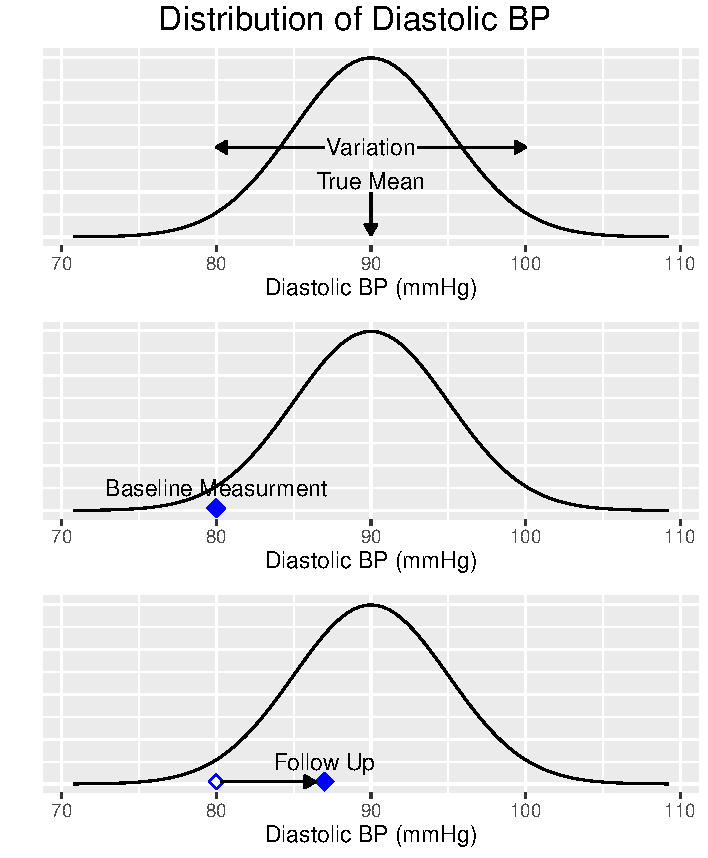
\includegraphics[scale=1]{DBP_plot}
	\caption{RTM effect in diastolic blood pressure in baseline and follow-up measurement with true mean and variation}
	\label{RTM_ex}
\end{figure}

Equation \ref{var} shows the unbiased estimator of population variance $\sigma^2$

\begin{equation}
	s^2=\sum_{i=1}^{n}\frac{\left(x_i-\bar{x}\right)}{n-1}
	\label{var}
\end{equation}

\chapter{Results and Discussion}


The $p$-value of $P(t_{(17)}>4.067)=0.000506$ and provide sufficient evidence that the treatment has a significant effect on increasing the weight of girls after removing the effect of RTM however the test doesn't quantify the amount of RTM. Further, all the methods overestimate the true effect of RTM and the proposed method is more close to the True value when the sample size is small as seen from a simulation study.



\begin{table}[H]
\centering
\caption{The total ${\hat T_l}\left( {c;n,\theta } \right)$, RTM ${\hat R_{l}}\left( {c;n,\theta } \right)$ and treatment ${\hat \psi_l }$ effects }
\begin{tabular}{ccccc}
	\hline
	& \multicolumn{4}{p{5cm}}{\centering Pre-post Measurement \\ of  treatment group (m=17) } \\ \cline{2-5} 
	Effects  &${\hat T_l}\left( {c;n,\theta } \right)$          & ${\hat R_{l}}\left( {c;n,\theta } \right)$          & ${\hat \psi_l }$       & p-value$^*$      \\ \hline
	Proposed &-7.248   &  1.476  & -5.772   & 0.00012                \\
	\cite{khan2022regression}     & -7.248        &  1.218        & -6.03       & 0.00016               \\ \hline
	\footnotesize{$^*$Adjusted for RTM}
	\label{effects}
	\end{tabular}
\end{table}


\chapter{Conclusion}
The summary of your work

\begin{appendices}
\chapter{R Codes}
\label{appA}
The following R functions return the scatter plot

\begin{lstlisting}[language=R]
# This is a comment in R
x <- c(1, 2, 3, 4, 5)
y <- c(6, 7, 8, 9, 10)
plot(x, y, main = "My Plot", xlab = "X Axis", ylab = "Y Axis")
\end{lstlisting}
	 
\chapter{Anorexia Patients Dataset}
Source: Brian Everitt (private communication)\\
These are weights, in pounds (lb), of young girls receiving three different treatments for
anorexia over a fixed period of time with the control group receiving the standard treatment.

\begin{center}
\begin{longtable}{cccccc}
\label{anorexia} \\
\hline
\multicolumn{2}{p{4cm}}{\centering Cognitive behavioral \\ treatment } & \multicolumn{2}{c}{\multirow{2}{*}{Control}} & \multicolumn{2}{c}{\multirow{2}{*}{Family therapy}} \\			\multicolumn{2}{c}{} & \multicolumn{2}{c}{}           & \multicolumn{2}{c}{}                               \\ \hline
\endfirsthead		
\multicolumn{6}{r}{{\textit{Continued on next page}}} \\ 
\endfoot
\hline
\endlastfoot			
Before  & After & Before    & After & Before    &   After\\ 
\hline
80.5    & 82.2  & 80.7  & 80.2  & 83.8  & 95.2  \\
84.9    & 85.6  & 89.4  & 80.1  & 83.3  & 94.3   \\
81.5    & 81.4  & 91.8  & 86.4  & 86    & 91.5   \\
82.6    & 81.9  & 74    & 86.3  & 82.5  & 91.9   \\
79.9    & 76.4  & 78.1  & 76.1  & 86.7  & 100.3  \\
88.7    & 103.6 & 88.3  & 78.1  & 79.6  & 76.7   \\
94.9    & 98.4  & 87.3  & 75.1  & 76.9  & 76.8  \\
...	    & ...   &...    & ...   & ...   &...    \\ \hline
\end{longtable}
\end{center}

\end{appendices}

\bibliography{bib_ref}
\addcontentsline{toc}{chapter}{References}
\bibliographystyle{apalike}
\end{document}